\chapter{Implementacija i korisničko sučelje}
		
		
		\section{Korištene tehnologije i alati}
		
			Komunikacija u timu realizirana je korištenjem aplikacije Discord\footnote[1]{https://discord.com/} te aplikacija WhatsApp\footnote[2]{https://www.whatsapp.com/}. Za izradu UML dijagrama korišten je
			web servis Visual Paradigm Online\footnote[3]{https://online.visual-paradigm.com/}, a kao sustav za upravljanje izvornim kodom Git\footnote[4]{https://git-scm.com/}. Udaljeni repozitorij projekta je dostupan na
			web platformi GitHub\footnote[5]{https://github.com/}.
			\smallbreak
			\noindent Kao razvojna okruženja korišteni su:
			\begin{itemize}
				\item IntelliJ IDEA Ultimate\footnote[6]{https://online.visual-paradigm.com/} - \textit{\textbf{backend}}
				\item Microsoft Visual Studio\footnote[7]{https://visualstudio.microsoft.com/} - \textit{\textbf{frontend, dokumentacija}}
			\end{itemize}
			\noindent Integrirana razvojna okruženja tvrtke JetBrains (1.), tj. Microsoft (2.).
			\smallbreak
			Aplikacija je napisana koristeći radni okvir Spring Boot\footnote[8]{https://spring.io/projects/spring-boot/} i jezik Java\footnote[9]{https://www.java.com/en/} za izradu 
			\textit{backend-a}, tj. radni okvir React\footnote[10]{https://reactjs.org/} i jezik JavaScript\footnote[11]{https://www.javascript.com/} za izradu \textit{frontend-a}.
			\smallbreak
			Baza podataka nalazi se na poslužitelju u oblaku DigitalOcean\footnote[12]{https://www.digitalocean.com/}.
			\eject 
		
	
		\section{Ispitivanje programskog rješenja}
			
			\subsection{Ispitivanje komponenti}

			\noindent Svi testovi napravljeni su pomoću JUnit, AssertJ i Mockito dependancy-a.
			\medbreak
			\noindent Za repliciranje kontrolera, servisa i repozitorija korištene su @MockBean, @Mock te @InjectMocks
			anotacije.
			\medbreak
			\noindent U svim testovima korišten je "Given-When-Then" način testiranja.
			\medbreak
			\noindent Za svaki test prikazan je dio izvornog koda (u obliku slike zbog preglednosti).
			Način nazivanja svake test funkcije prikazuje gdje se testira, što se testira te koji se povratni
			rezulat očekuje.
			\eject
			
			\noindent\textbf{AuthorizationControllerTest}
			\begin{figure}[H]
				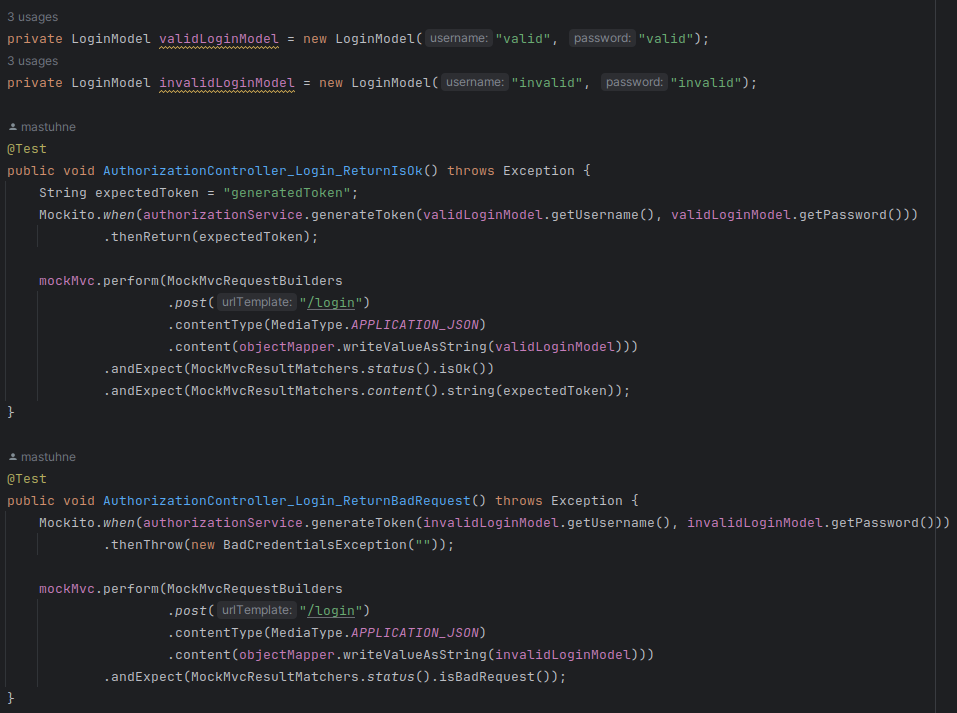
\includegraphics[scale=0.45]{slike/auth_controller_test.png}
				\centering
				\caption{AuthorizationControllerTest kod}
				\label{fig:authtest}
			\end{figure}

			\noindent\textbf{RecipeControllerTest}
			\begin{figure}[H]
				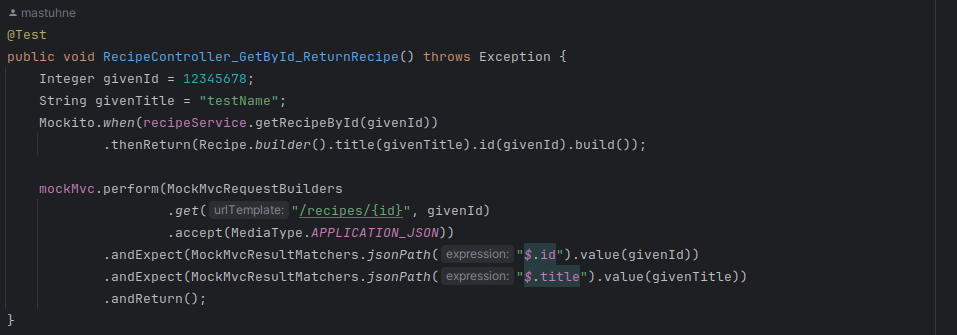
\includegraphics[scale=0.45]{slike/recipe_controller_test.png}
				\centering
				\caption{RecipeControllerTest kod}
				\label{fig:reccontrolltest}
			\end{figure}

			\eject
			\noindent\textbf{CategoryServiceTest}
			\begin{figure}[H]
				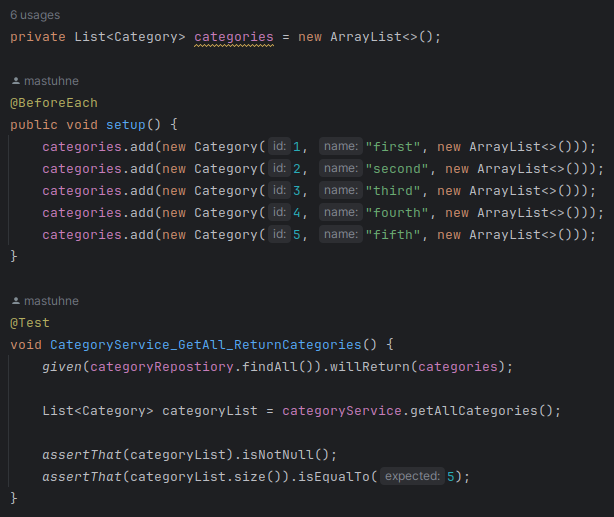
\includegraphics[scale=0.5]{slike/category_service_test.png}
				\centering
				\caption{CategoryServiceTest kod}
				\label{fig:cattest}
			\end{figure}

			\noindent\textbf{RecipeServiceTest}
			\begin{figure}[H]
				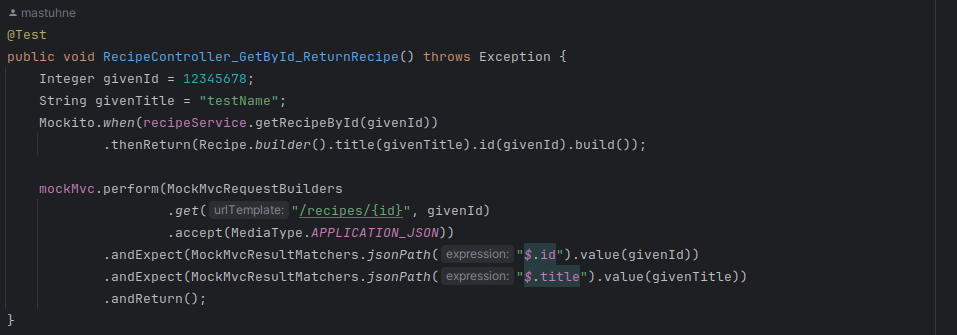
\includegraphics[scale=0.5]{slike/recipe_controller_test.png}
				\centering
				\caption{RecipeServiceTest kod}
				\label{fig:recest}
			\end{figure}

			\eject
			\noindent\textbf{UserRepositoryTest}
			\begin{figure}[H]
				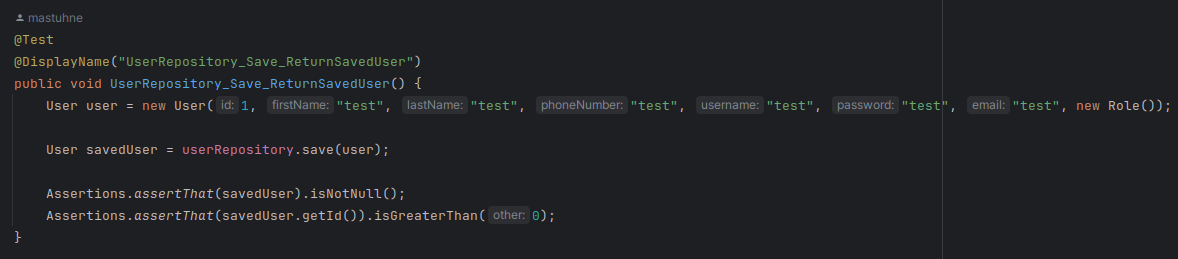
\includegraphics[scale=0.4]{slike/user_repository_test.png}
				\centering
				\caption{UserRepositoryTest kod}
				\label{fig:userretest}
			\end{figure}

			\noindent\textbf{Prikaz rezultata testova:}
			\begin{figure}[H]
				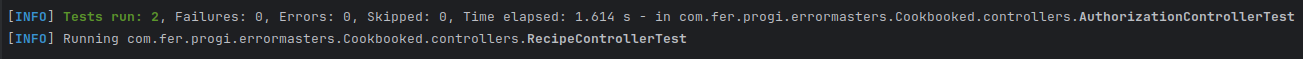
\includegraphics[scale=0.38]{slike/test_auth_con_res.png}
				\centering
				\caption{Rezultat AuthorizationControllerTest-a}
				\label{fig:authconres}
			\end{figure}
			\begin{figure}[H]
				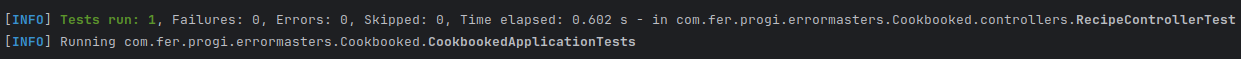
\includegraphics[scale=0.4]{slike/test_rec_con_res.png}
				\centering
				\caption{Rezultat UserRepositoryTest-a}
				\label{fig:recconres}
			\end{figure}
			\begin{figure}[H]
				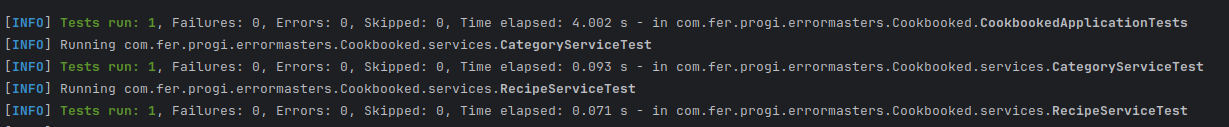
\includegraphics[scale=0.4]{slike/test_three_res.png}
				\centering
				\caption{Rezultat ... testa}
				\label{fig:threeres}
			\end{figure}
			\begin{figure}[H]
				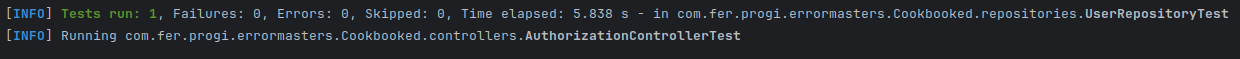
\includegraphics[scale=0.4]{slike/test_user_repo_res.png}
				\centering
				\caption{Rezultat UserRepositoryTest-a}
				\label{fig:userrepores}
			\end{figure}
			\begin{figure}[H]
				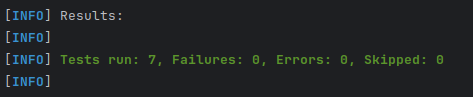
\includegraphics[scale=0.4]{slike/test_all_res.png}
				\centering
				\caption{Rezultat svih testova}
				\label{fig:allres}
			\end{figure}
			\eject




			
			\subsection{Ispitivanje sustava}
	
			\begin{figure}[H]
				
\includegraphics[scale=0.4]{slike/error404.png}
				\centering
				\caption{Selenium}
				\label{fig:selenium}
			\end{figure}
			
			\eject 
		
		
		\section{Dijagram razmještaja}

			 \noindent Dijagram razmještaja prikazuje fizički razmještaj programskih artefakata 
			 na fizičkoj ili virtualnoj infrastrukturi. Na platformi DigitalOcean implementirano je
			 rješenje koje koristi Docker kontejnere za ispunjavanje pozadinske funkcionalnosti 
			 web aplikacije. Klijenti koriste web preglednik kako bi pristupili web applikaciji.
			 Sustav je baziran na arhitekturu "klijent-poslužitelj", dok je komunikacija između 
			 računala korisnika i računala poslužitelja ostvarena putem HTTP veze.
			

			\begin{figure}[H]
				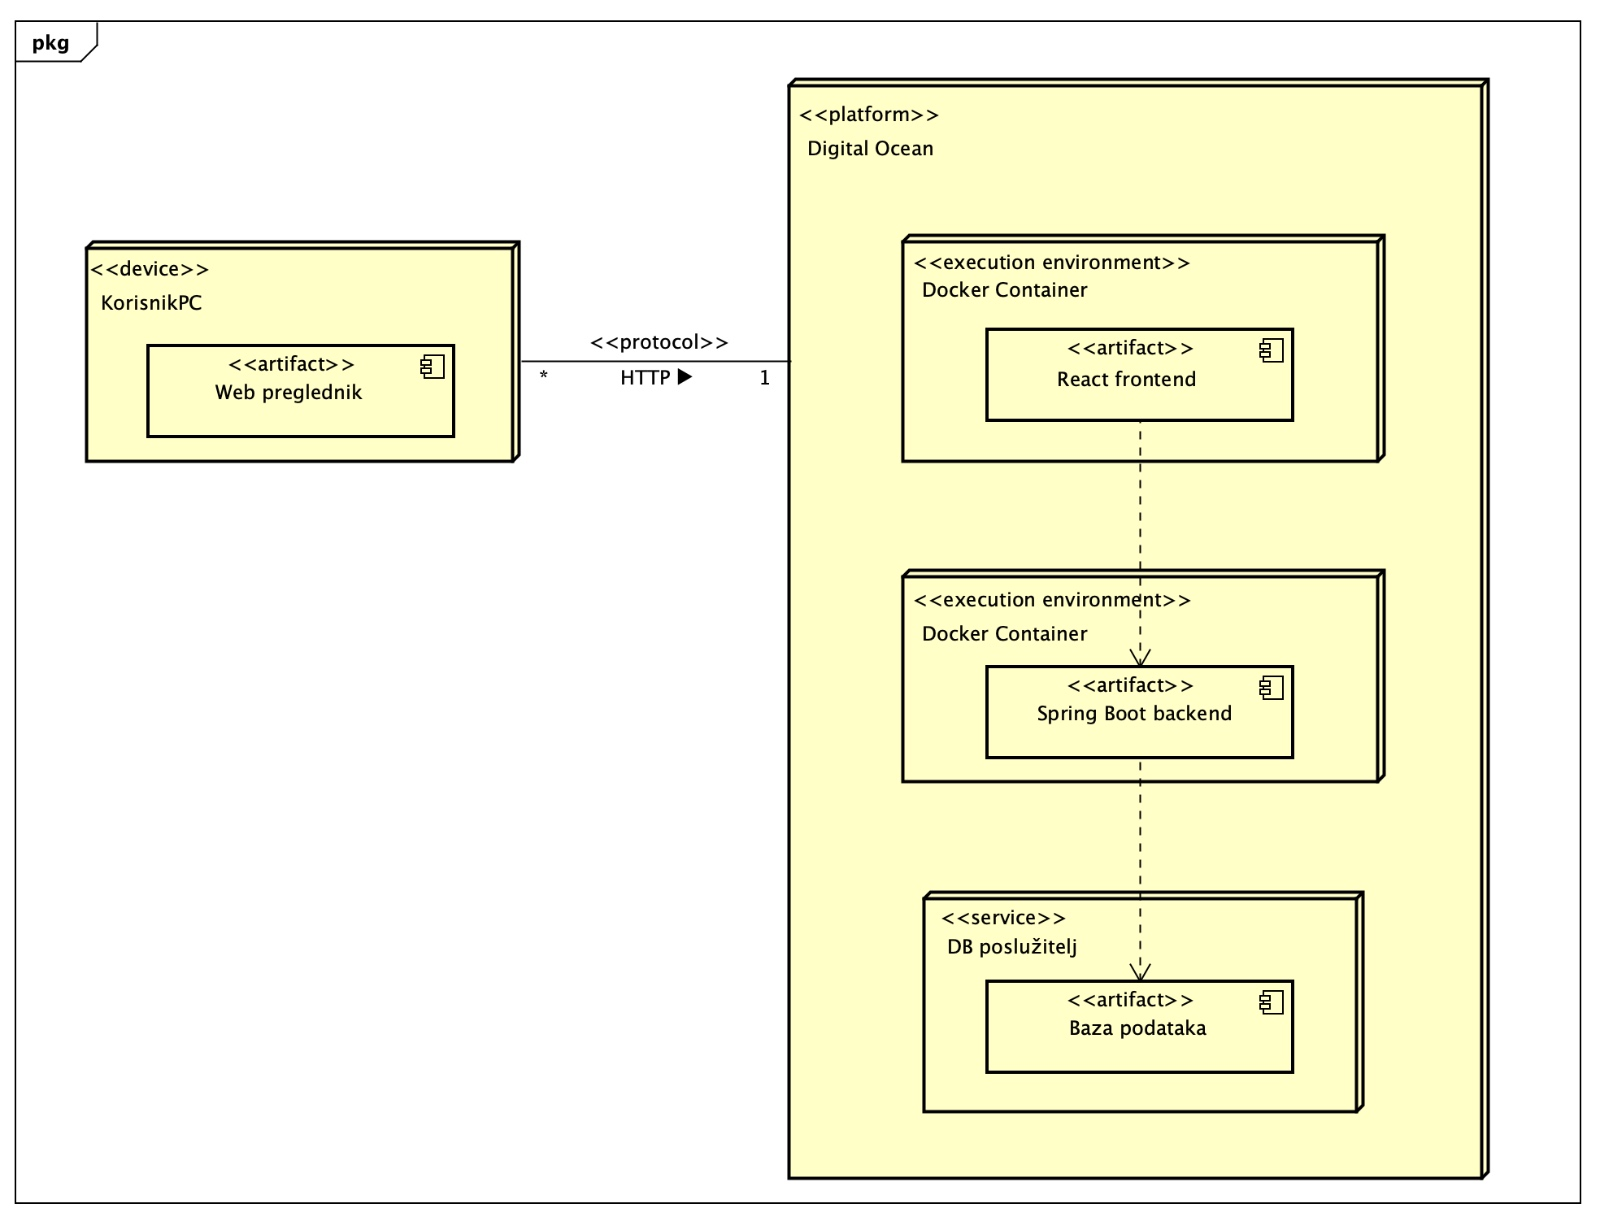
\includegraphics[scale=0.28]{dijagrami/dijagram_razmjestaja.jpeg}
				\centering
				\caption{Dijagram aktivnosti}
				\label{fig:bpdiag}
			\end{figure}
			\eject 
		
		\section{Upute za puštanje u pogon}
			\noindent \textbf{Instalacija i konfiguracija baze podataka}
			\noindent Potrebno je otići na platformu koja nudi usluge poslužitelja baze podataka, 
			u našem slučaju, \textit{DigitalOcean}. Također, odlučili smo se koristiti PostgreSQL
			za pohranu podataka.

			\noindent Kod stvaranja baze podataka treba odabrati slijedeće postavke:
			\begin{itemize}
				\item Regija podatkovnog centra (data center region) – Amsterdam
				\item Baza podataka – PostgreSQL v15
				\item CPU – Regular
				\item Plan – 1vCPU, 2 GB RAM
			\end{itemize}

			\begin{figure}[H]
				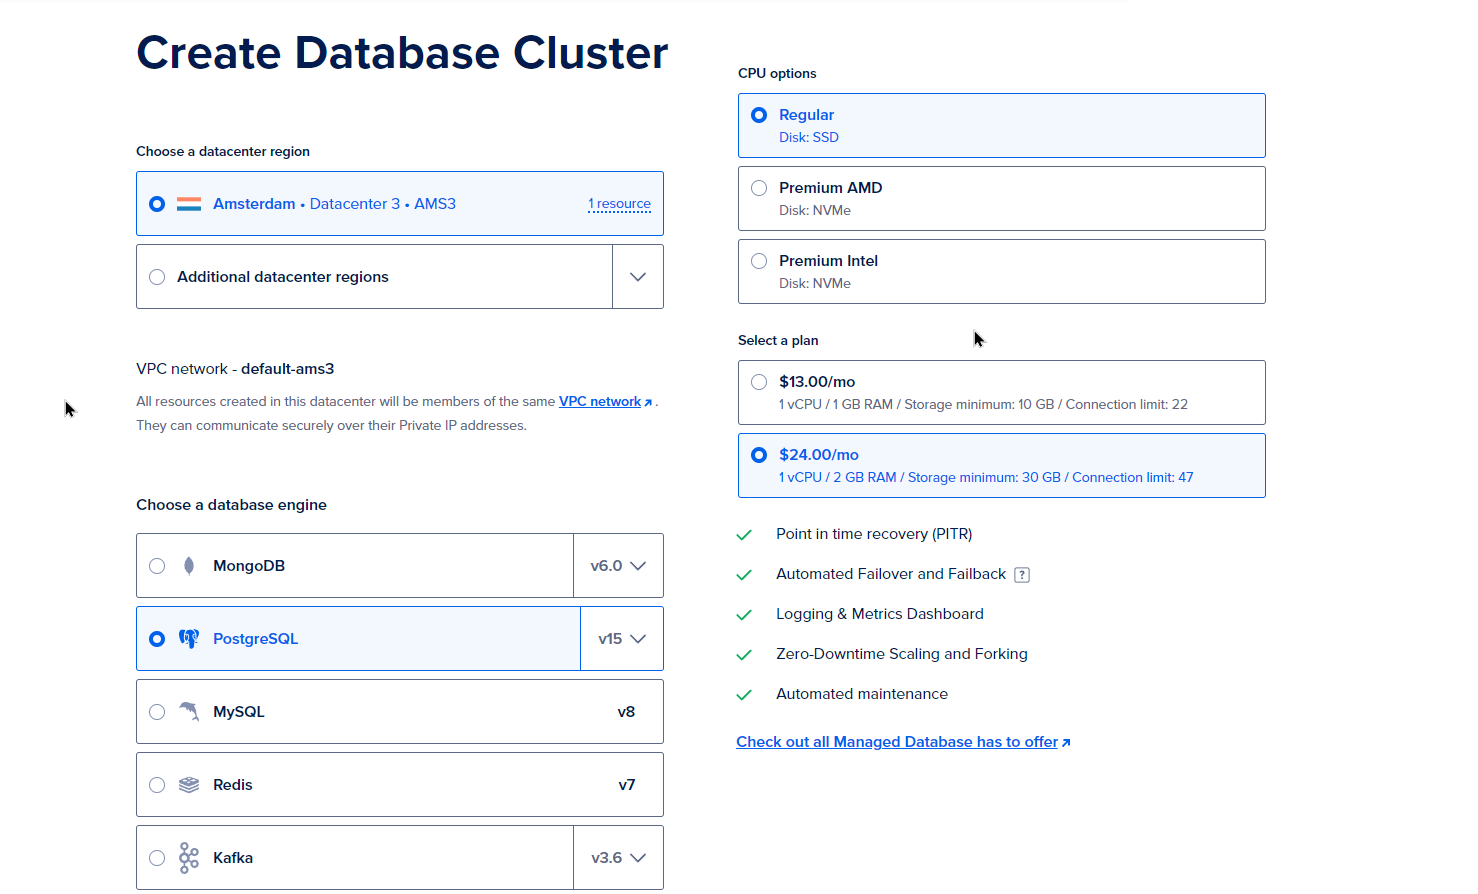
\includegraphics[scale=0.4]{slike/conf_base.png}
				\centering
				\caption{Konfiguracija baze podataka}
				\label{fig:baseconf}
			\end{figure}

			\noindent Nakon uspješnog stvaranja baze podataka platforma će nas proslijediti na stranicu
			na kojoj možemo provesti dodatnu konfiguraciju baze podataka. Na toj se stranici
			nalaze upute za spajanje (na bazu), koje ćemo iskoristiti kako bismo dobili izravan
			pristup bazi.

			\begin{figure}[H]
				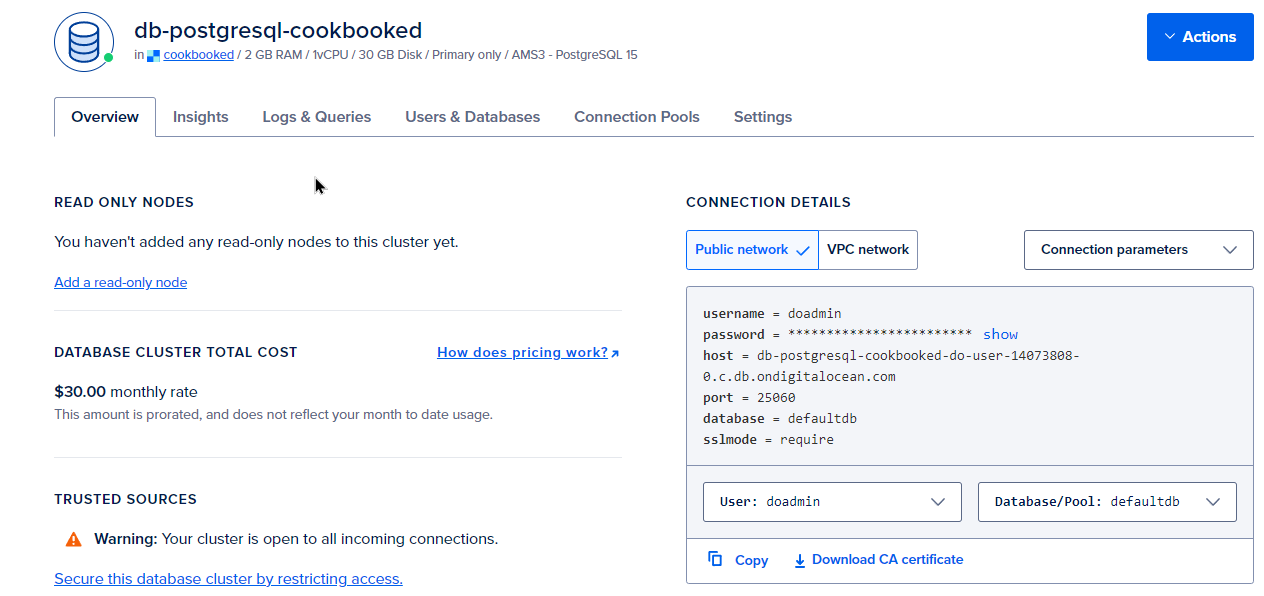
\includegraphics[scale=0.4]{slike/add_conf_base.png}
				\centering
				\caption{Dodatna konfiguracija baze podataka}
				\label{fig:addbaseconf}
			\end{figure}

			\eject
			\noindent \textbf{Spajanje na bazu podataka}

			\noindent Spajanje na bazu provodimo putem okoline za upravljanje bazom podataka.
			U našem slučaju koristili smo \textit{JetBrains}-ov alat \textit{DataGrip}.
			Navigacijom na \textit{Database Explorer} odabiremo opciju \textit{New} te u padajućem
			izborniku odaberemo opciju \textit{Data Source - PostgreSQL}. U otvorenom prozoru
			unosimo podatke koje smo dobili kao povratnu informaciju prilikom kreiranja i konfiguriranja
			baze podataka.

			\begin{figure}[H]
				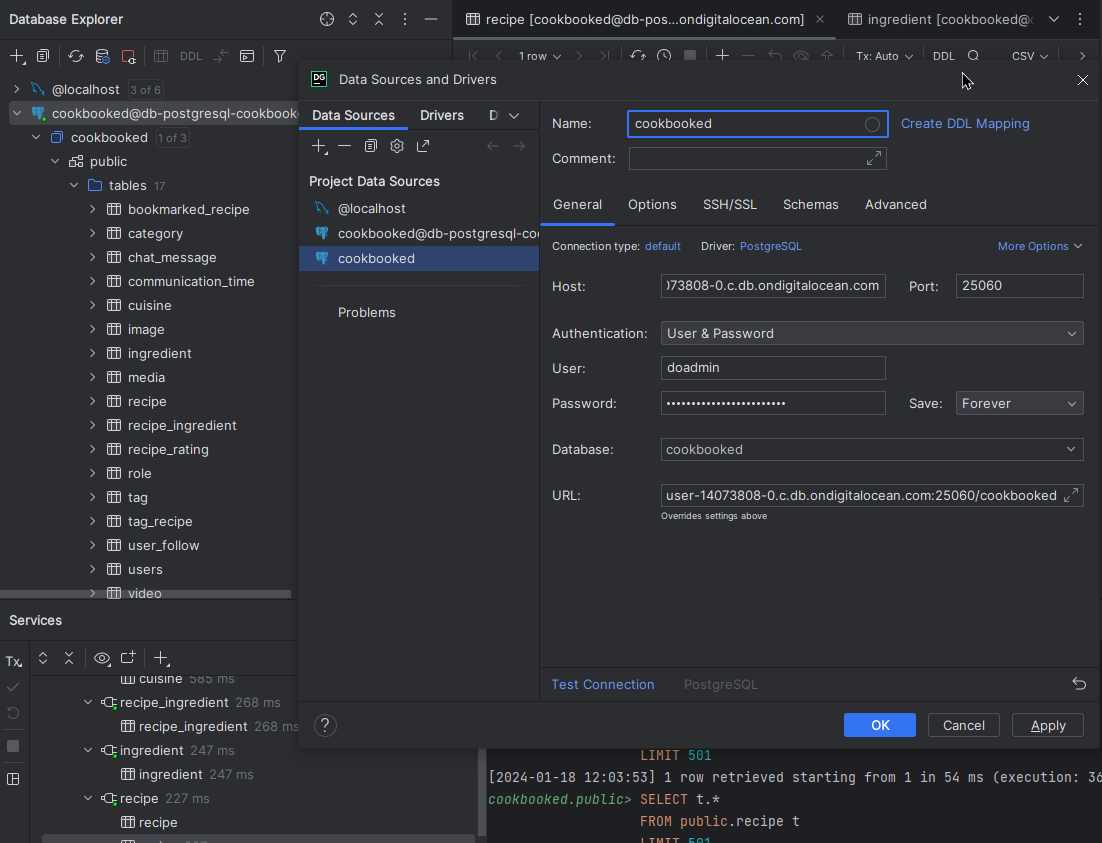
\includegraphics[scale=0.4]{slike/conn_base.png}
				\centering
				\caption{Spajanje pomoću alata \textit{DataGrip}}
				\label{fig:conbase}
			\end{figure}

			\noindent Kopirat ćemo URL, tj. JDBC URL koji ćemo kasnije upisati u \textit{Spring Boot application
			properties} datoteku.

			\noindent Pritiskom gumba "OK" stvara se novi unos u \textit{Database Explorer}. Također, klikom na gumb
			"Test Connection" možemo testirati jesmo li sve podatke unijeli ispravno.

			\eject
			\noindent \textbf{Punjenje baze podataka}

			\noindent Odabirom unesene baze u \textit{Database Explorer}-u možemo pronaći public shemu koja će
			biti glavno spremište naših podataka. Klikom desne tipke miša na public shemu, biti će prikazan
			izbornik u kojem odabiremo opciju \textit{SQL Scripts - Run SQL Script}. Otvoriti će se nova kartica
			u kojoj ćemo staviti sadržaj "cookbooked.sql" datoteke koja predstavlja opis strukturnog modela baze.
			
			\medbreak
			\noindent \textbf{Konfiguracija \textit{Spaces Object Storage-a} za spremanje multimedijskih datoteka}
			
			\noindent Za pohranu slika i videa koristimo \textit{DigitalOcean}-ov \textit{Spaces Object Storage}.
			Kofiguracija zahtjeva da odaberemo:
			
			\begin{itemize}
				\item Regiju – izaberemo najbliži server
				\item CDN – uključen
				\item Ime
			\end{itemize}

			\noindent Nakon što smo kreirali \textit{Spaces Bucket}, biti će nam potreban \textit{API-key} za taj
			\textit{bucket}, kako bismo ga mogli koristiti na \textit{Spring Boot backend}-u.
			\textit{API-key} ćemo dobiti odabirom opcije \textit{API - Spaces Key} u izborniku platforme
			\textit{DigitalOcean}. Tamo ćemo izgenerirati naše API ključeve.

			\begin{figure}[H]
				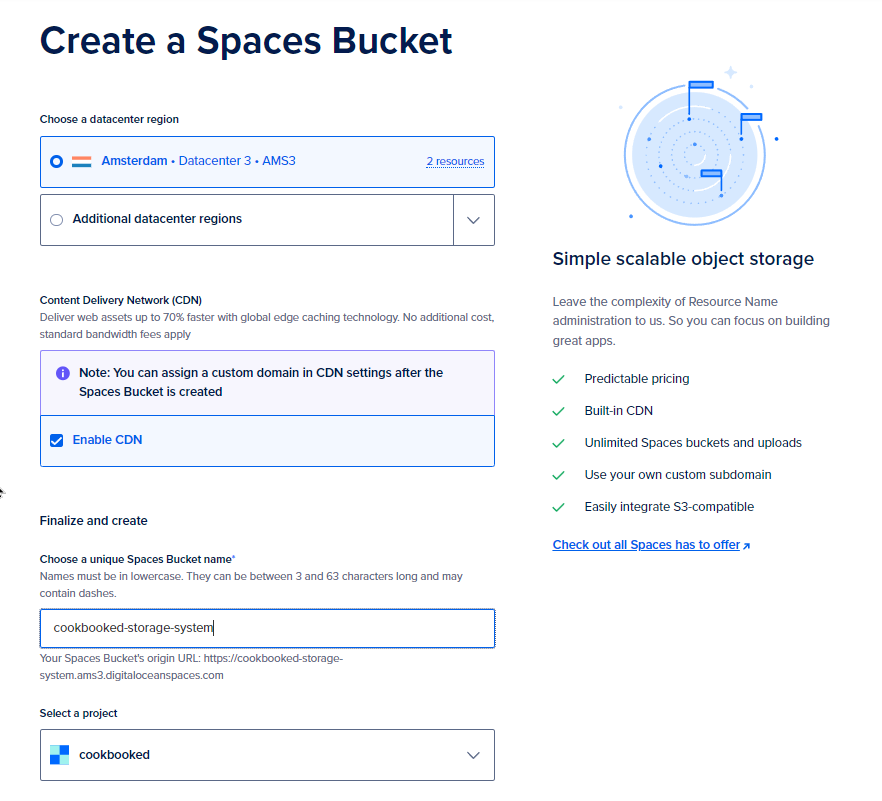
\includegraphics[scale=0.4]{slike/spaces_bucket.png}
				\centering
				\caption{Kreiranje \textit{Spaces}}
				\label{fig:createspaces}
			\end{figure}
			
			\eject
			\noindent \textbf{Instalacija i konfiguracija Spring Boot-a}
			\noindent Nakon uspješnog konfiguriranja baze podataka i \textit{Spaces}-a, potrebno je klonirati repozitorij
			aplikacije \textbf{CookBooked}. U direktoriju naziva \textit{backend} potrebno je konfigurirati
			\textit{application.properties} datoteku.

			Potrebno je:

			\begin{itemize}
				\item postaviti spring.datasource.url
				\item postaviti spring.datasource.username
				\item postaviti spring.datasource.password
				\item postaviti s3.acces.key, s3.secret.key, s3.server.url, s3.bucket.name, s3.bucket.region
			\end{itemize}

			\begin{figure}[H]
				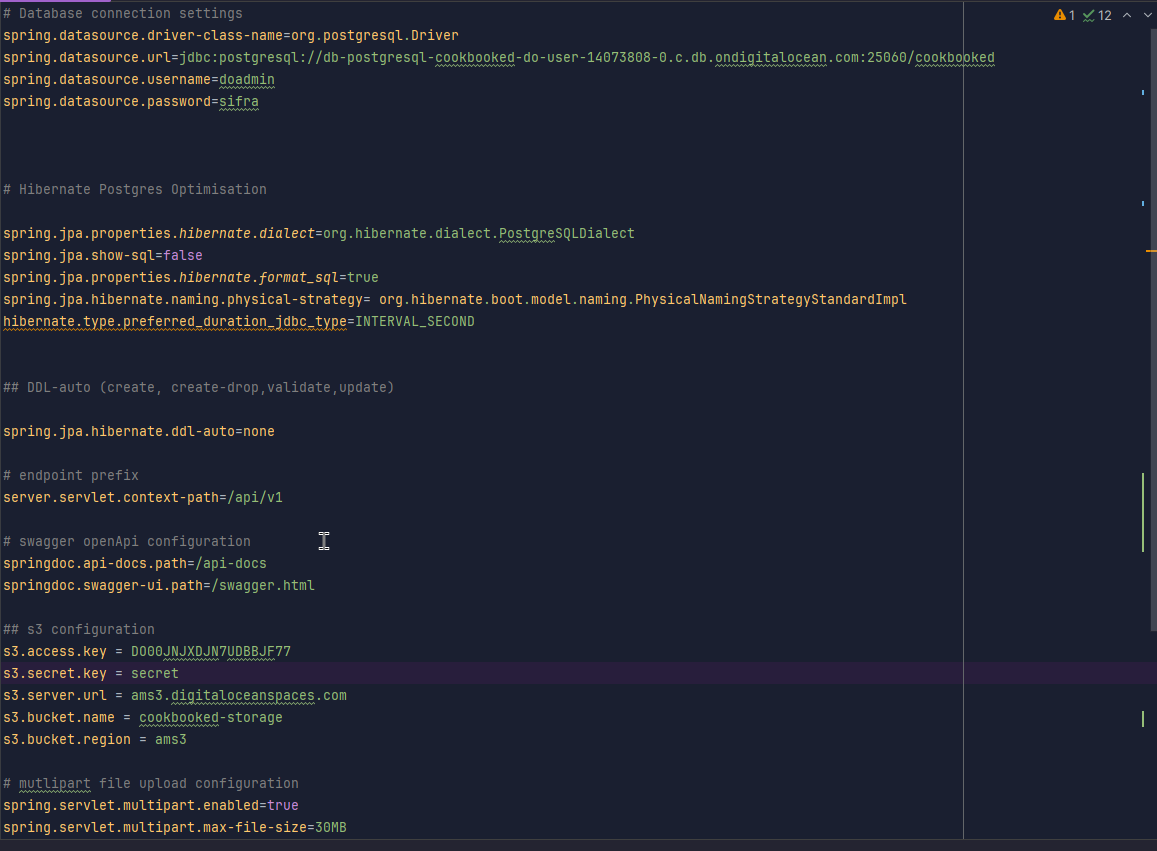
\includegraphics[scale=0.4]{slike/app_prop.png}
				\centering
				\caption{Izgled \textit{application.properties} datoteke}
				\label{fig:approp}
			\end{figure}


			\noindent Backend REST API-server je tada spreman te ga možemo pokrenuti naredbom
			\textbf{./mvnw spring-boot:run}. Nakon izvršavanja naredbe, \textit{backend} je pokrenut na
			\textit{port}-u 8080.

			\eject
			\noindent \textbf{Instalacija i konfiguracija REACT frontend-a}

			\noindent \textit{Frontend} je potrebno konfigurirati da šalje zahtjeve na \textit{backend} server.
			To ćemo postići tako da u \textbf{.env} datoteci postavimo IP adresu ili domenu \textit{backend}
			servera. Nakon toga moguće je pokrenuti naredbe \textbf{npm install} koja će učitati
			potrebne biblioteke, \textbf{npm build} koja će "izgraditi" našu aplikaciju te \textbf{npm run}
			koja će pokrenuti aplikaciju. 
		
		
			\eject 